% =====================================================================
%  hg.tex — NỘI DUNG BÁO CÁO (chỉ phần thân, KHÔNG có preamble)
%  Dùng trong main.tex:   \input{content/hg}
%  Cần nạp trước trong preamble của main.tex:  \input{content/preamble_hg}
%  Đường dẫn ảnh "figures/..." tính từ thư mục chứa main.tex.
% =====================================================================
% =====================================================================
\section{Phương pháp}
% =====================================================================

Mỗi ảnh $28\times28$ được làm phẳng thành vector $\mathbf{x}\in[0,1]^{D}$ với $D=784$ (giá trị pixel chia 255). Nhãn $y\in\{0,\dots,9\}$, $K=10$ lớp. Phần này trình bày chi tiết hai phương pháp do nhóm phụ trách là Multinomial Naive Bayes và Random Forest; Logistic Regression và MLP được tóm tắt ở mục~\ref{sec:exp}.

% ---------------------------------------------------------------------
\subsection{Multinomial Naive Bayes}
 
\paragraph{Mô hình.} Naive Bayes chọn lớp có xác suất hậu nghiệm lớn nhất theo định lý Bayes, với giả định các pixel độc lập có điều kiện khi biết lớp:
\begin{equation}
\hat y=\argmax_{c}\,P(c\mid\mathbf{x})=\argmax_{c}\,P(c)\prod_{j=1}^{D}P(j\mid c)^{x_j}.
\end{equation}
Mô hình đa thức coi ảnh như một ``túi mực'': cường độ $x_j$ là số lần ``nét mực'' rơi vào pixel $j$, và $\theta_{cj}=P(j\mid c)$ là xác suất một đơn vị mực của lớp $c$ rơi vào pixel $j$, với $\sum_j\theta_{cj}=1$. Cường độ là số thực trong $[0,1]$ chứ không phải số đếm nguyên, nhưng công thức ước lượng vẫn áp dụng được (``số đếm phân số'').
 
\paragraph{Ước lượng tham số.} Gọi $n_c$ là số ảnh của lớp $c$ và $N_{cj}=\sum_{i:y_i=c}x_{ij}$ là tổng mực tại pixel $j$ của lớp đó. Xác suất tiên nghiệm và xác suất pixel có làm trơn Laplace hệ số $\alpha>0$:
\begin{equation}
\pi_c=\frac{n_c}{n},\qquad
\theta_{cj}=\frac{N_{cj}+\alpha}{\sum_{j'}N_{cj'}+\alpha D}.
\end{equation}
Làm trơn tránh $\theta_{cj}=0$ cho các pixel không bao giờ sáng ở một lớp (EDA cho thấy 67/784 pixel luôn bằng 0 trên toàn tập train); nếu không, chỉ một pixel ``lạ'' cũng đưa xác suất của cả lớp về 0.
 
\paragraph{Dự đoán trong miền log.} Tích của 784 xác suất nhỏ gây tràn dưới, nên mọi phép tính được đưa về log:
\begin{equation}
s_c(\mathbf{x})=\log\pi_c+\sum_{j=1}^{D}x_j\log\theta_{cj},\qquad
\hat y=\argmax_c s_c,\qquad
P(c\mid\mathbf{x})=\frac{e^{s_c}}{\sum_{k}e^{s_k}}.
\end{equation}
Xác suất hậu nghiệm được chuẩn hoá bằng softmax ổn định số (trừ $\max_k s_k$ trước khi lấy mũ).
 
\begin{algorithm}[H]
\caption{Multinomial Naive Bayes}\label{alg:nb}
\begin{algorithmic}[1]
\Function{Fit}{$X\in\R^{n\times D}$, $\mathbf{y}$, $\alpha$}
  \For{mỗi lớp $c$}
    \State $X_c\gets$ các hàng của $X$ có nhãn $c$
    \State $\log\pi_c\gets\log(|X_c|/n)$
    \State $\mathbf{N}_c\gets\sum_{\text{hàng}}X_c$ \Comment{vector $D$ chiều}
    \State $\log\boldsymbol\theta_c\gets\log\big((\mathbf{N}_c+\alpha)/(\textstyle\sum\mathbf{N}_c+\alpha D)\big)$
  \EndFor
\EndFunction
\Function{Predict}{$X$}
  \State $S\gets X\,(\log\Theta)^{\top}+\log\boldsymbol\pi$ \Comment{$S\in\R^{n\times K}$, một phép nhân ma trận}
  \State \Return $\argmax$ theo từng hàng của $S$ \quad (hoặc $\mathrm{softmax}(S)$ cho xác suất)
\EndFunction
\end{algorithmic}
\end{algorithm}
 
\paragraph{Chi tiết cài đặt} (\code{naive\_bayes.py}).
Lớp \code{MultinomialNB(alpha)} lưu \code{log\_prior} (kích thước $K$) và \code{log\_feature\_prob} (kích thước $K\times D$). Huấn luyện chỉ cần một vòng lặp qua $K$ lớp với các phép cộng vector, độ phức tạp $O(nD)$. Dự đoán cho cả tập là một phép nhân ma trận \code{X @ log\_feature\_prob.T + log\_prior}, chi phí $O(DK)$ mỗi ảnh. Dữ liệu được ép về \code{float64} trong \code{fit} để tổng $N_{cj}$ trên hàng nghìn ảnh không bị sai số làm tròn của \code{float32}. Nhãn lớp được lưu trong \code{classes} nên \code{predict} trả về nhãn gốc. Mô hình sau huấn luyện chỉ chiếm 0.1\,MB.
 
\paragraph{Cách kiểm chứng.}
\begin{enumerate}
\item \textbf{Đối chiếu tham số với scikit-learn}: huấn luyện lớp \code{MultinomialNB(alpha=1)} của scikit-learn trên cùng dữ liệu \code{float64}, kiểm tra bằng \code{np.allclose} rằng \code{log\_feature\_prob} trùng \code{feature\_log\_prob\_}, \code{log\_prior} trùng \code{class\_log\_prior\_}, \code{predict\_proba} trùng trên tập validation, và tỉ lệ dự đoán trùng nhau là 100\%. Vì công thức xác định (không có ngẫu nhiên), yêu cầu là khớp \emph{tuyệt đối}, không chỉ gần nhau về accuracy.
\item \textbf{Kiểm tra trực quan}: vẽ $\boldsymbol\theta_c$ thành ảnh $28\times28$ (phải giống ``ảnh trung bình'' của chữ số $c$) và bản đồ $\log\boldsymbol\theta_7-\log\boldsymbol\theta_1$ để xem pixel nào ``bỏ phiếu'' cho 7 so với 1. Kết quả ở Hình~\ref{fig:nb_theta}: mỗi $\boldsymbol\theta_c$ là một chữ số mờ đúng hình dạng; trên bản đồ $7-1$, vùng đỏ (ủng hộ 7) nằm ở hai bên và phần đáy ảnh, nơi chữ 1 hầu như không có mực, còn vùng xanh (ủng hộ 1) chạy dọc đường chéo giữa ảnh, trùng với nét của chữ 1.
\end{enumerate}
 
\begin{figure}[H]
\centering
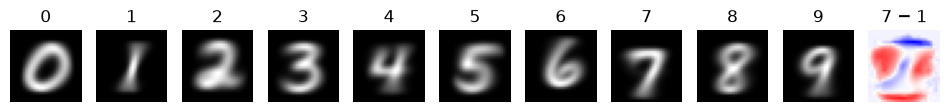
\includegraphics[width=0.95\textwidth]{figures/nb_theta.png}
\caption{Tham số $\boldsymbol\theta_c$ của Multinomial NB vẽ thành ảnh $28\times28$ cho 10 lớp, và hiệu $\log\boldsymbol\theta_7-\log\boldsymbol\theta_1$ (đỏ: ủng hộ 7, xanh: ủng hộ 1).}\label{fig:nb_theta}
\end{figure}

